\documentclass{article}

\usepackage{graphicx,color,tabularx,amsmath,amssymb,fancyvrb,soul}
\usepackage{subcaption}
\usepackage{float}

\begin{document}

\section{Abstract}

\section{Introduction}

\subsection{Project Motivation}

This project was motivated by two key factors. 

\subsection{Problem Outline}



\subsection{Project Specification}



\subsection{Report Structure}

\section{Background}

There are two main GCSE Mathematics revision tools in use today. The first tool is MyMaths[4] which is a website which aims to enrich a student's classroom learning experience. MyMaths main use case is to supplement the material covered in class by a teacher. The main feature of MyMaths is the online homework feature. This feature enables teachers to set homework to their class. This homework covers a specific topic, for example Venn diagrams, and the students can answer questions on this topic. Example homework questions on the topic of Venn diagrams can be viewed as figure \ref{figure:mymathsHomeworkQuestion1}.
\begin{figure}[H]
	\centering
	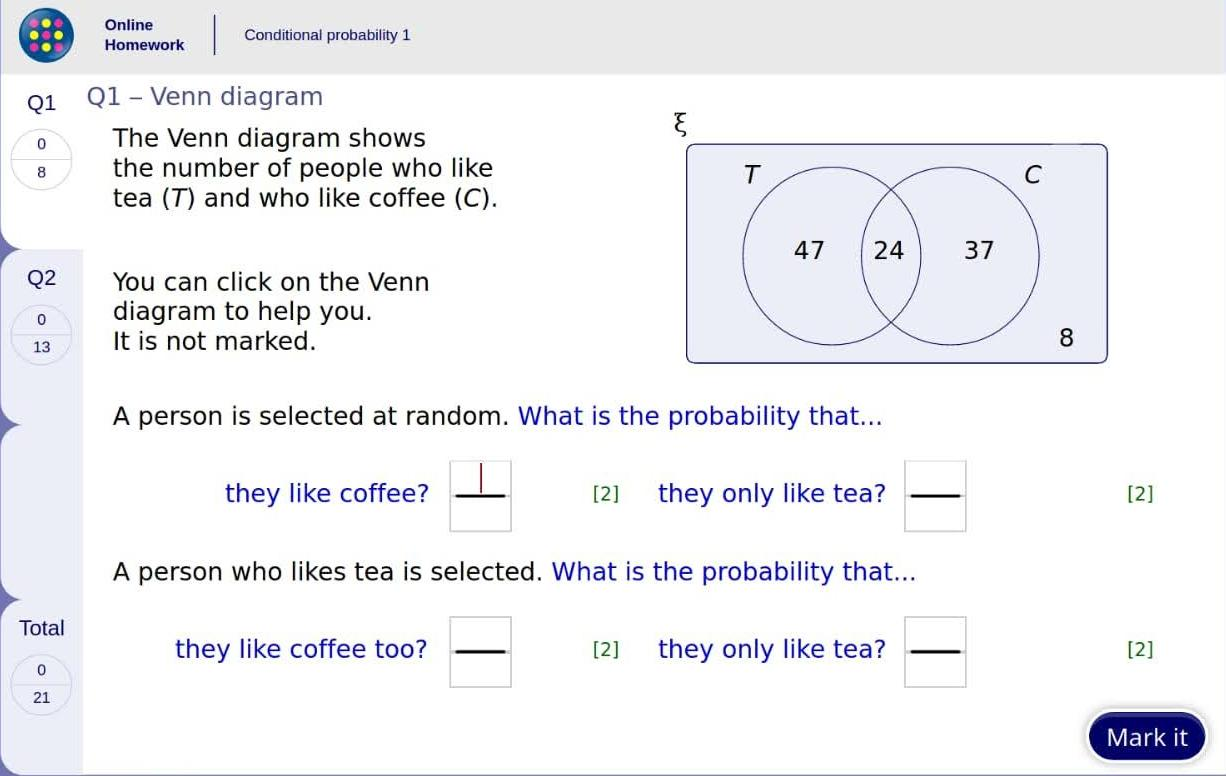
\includegraphics[width=0.9\linewidth]{./data/mymathsQuestion1.jpg}
	\caption{Venn diagram homework questions.}
	\label{figure:mymathsHomeworkQuestion1}
\end{figure}
The student's scores are then generated (as a percentage) and sent back to the teacher. \\

The values selected in the homework are unique each time a student attempts that specific homework. This prevents a student from memorizing a specific answer to pass the homework. A teacher can also see the number of attempts that a student has currently taken for the homework, and their highest score. Giving a teacher the ability to see the number of attempts that a student has at questions on a particular topic highlights where a student is struggling and can enable one on one teaching to boost the student's knowledge in that particular topic. A student can also attempt a homework which has not been set by their teacher. This allows a student to revise any topic in GCSE Mathematics on their own without a teacher. \\

MyMaths also gives a student the ability to take a lesson in any topic in GCSE Mathematics. This lesson walks through an example question in the topic, and then provides practice questions which are of a similar style to the homework questions. These questions are then marked, and where the student answers the question incorrectly, the correct answer is displayed next to the answer box. \\

MyMaths, however, is intended to be used in a web browser, and so is designed to be used on a desktop computer or a laptop. Due to the increase in smartphone adoption, more people of GCSE age have access to smartphones on a regular basis [x]. 
% find this figure somewhere
MyMaths has an iOS and Android application for tablets, but not a specific application for smartphones[5]. This prevents students who own their own smartphones but do not have access to a tablet on a regular basis from revising using MyMaths. \\

The second main GCSE Mathematics revision tool is Khan Academy[6] which is a non-profit organization which aims to "provide a free, world-class education for anyone, anywhere"[6]. 

\section{Methodology}

Initially, the project was going to have a waterfall based approach to software development. This, however, was not the best way to go about software development in this situation. 

%Go into detail about the scrum methodology.

\section{Design}



% Discuss the control flow of the program, why it works the way it does etc...
% Get the control flow diagram from the presentation and discuss how pages are connected
% Make a new diagram, a more impressive one, which also shows the information transfer between the 
% separate activities.

\section{Implementation}

\subsection{Questions}



\section{Project Management}

This project was a large software engineering project, especially for a team size of one. This meant that effective project management was required to keep the project going and make it a success. 

\subsection{Schedule}

A schedule was created early, and updated throughout the project to represent and handle the amount of work which had been completed. Two key versions of the schedule were displayed to various stakeholders throughout the project in key documents. These key documents were the project specification and the progress report. 

\subsubsection{Project Specification Schedule}

At the beginning of this project a schedule was created. This schedule aimed to complete all of the requirements created in the project specification[x]. The schedule was created using a technique common in industry which involved some numbered cards. Each requirement was reviewed. Each review consisted of analysing the relative difficulty of the requirement with respect to all of the other requirements. The difficulty was quantified using the numbered cards, the cards would follow a logarithmic pattern, doubling with difficulty each time. The lowest card was 1/4 and the largest was 16. Any requirement larger than 16 was then broken down into sub-requirements, these sub-requirements would then in turn be broken down if they were above 16 difficulty. \\

This relative difficulty in requirements was used to create a rough schedule for the project, assuming all requirements would be completed. This schedule was the one included in the original project specification. This schedule can be seen as a Gantt chart in figure[x].

\subsubsection{Progress Report Schedule}

The progress report submitted on 24\textsuperscript{th} November 2019 updated this schedule, once it was realised that development was slower than initially intended through term one of this academic year (October 2019 - December 2019) due to personal reasons. The new schedule, referred to from now on as the Christmas schedule, again made the assumption that every requirement would be completed before the deadline. To mitigate against the slow development conducted through term one, the Christmas schedule increased the workload of the project throughout the Christmas period (8\textsuperscript{th} December 2019 - 8\textsuperscript{th} January 2020) and throughout term two of the project. 

\subsubsection{Schedule Evaluation}

The image displayed below as figure [x] is an assessment of the completion of the final requirements in respect to the project specification schedule. 


\subsection{Tools}

This project utilized several tools to aid in the development of this Android application. Two of the main tools used to add value to this project are outlined below, one from a development point of view and one from a project management standpoint. 

\subsubsection{Android Studio}

Android Studio was used as an IDE (Integrated Development Environment) throughout development as it comes with many useful built in features. These features are specifically designed with android app development in mind. Examples of these features are: 

\begin{itemize}
	\item Rendering engine which converts XML into how it will appear in the application itself
	\item Android phone emulator
\end{itemize}

The rendering engine enables both the ability to edit the XML tags and see the effects in real time, as well as the ability to edit directly into the rendering engine with a drag and drop feature. This enables quick prototyping for new pages through the use of the drag and drop feature whilst also allowing a much larger degree of control through the ability to directly edit the XML.\\

Use of the android phone emulator enabled quick and efficient testing cycles. When a feature was initially developed, it could be tested on a wide range of devices through the phone emulator. This add on enabled the emulation of any modern phone through the ability to download files specific to that device. The app could then be tested on an accurate test bed, seeing how the app would look and work on a mobile device. Tablets could also be emulated, which helped with ensuring the application worked on a wide variety of devices.\\

The Android Studio IDE greatly increased the efficiency of development. This was encouraged through the notion that it was only designed specifically for android development, and so could focus entirely on that. Being built upon the IntelliJ platform meant that code editing was incredibly smooth and intuitive. \\

\subsubsection{Git}

Git was used as version control for this project. This enabled access to the project from any device, anywhere, anytime. It also enabled the ability to revert back to an earlier version of the project if something went wrong. This meant that development could take place without fear of failure, as if anything went wrong the project could just be reverted to the last working state.\\

The repository for this project can be found at[x]. This repository is public and can be accessed by anyone. This enables anyone to see the code that would be running on their machines.\\

Git also logs the time when a change is made to the code. This enabled precise tracking of requirement completion and aided project management. Git commit messages for this project were all deliberately helpful. Git commit messages were written so that they would explain the changes made to the codebase, so they could be logs of when project requirements were completed. The git commit messages for this project can be viewed and give a detailed timeline of when requirements were completed and features were added. This was incredibly useful as it gave updates of any changes made to the codebase as soon as it was available to anyone who follows the repository, and also was used to create a timeline of when requirements were completed for this final report. \\

% Move into the methodology section. Certainly the information about the notes file.
\subsection{Weekly Work????}

Weekly meetings were held with the project supervisor to keep key stakeholders in the project up to date with development. Alongside weekly meetings, access was given to the project supervisor to the  github repository early in development. This enabled the project supervisor to directly monitor completed work. \\

A document in the github repository called notes.txt is a file which was edited after every development session was completed. This file contained notes on what was intended to be completed during each development session, as well as what was actually completed. A substantial amount of time was spent at the beginning of early development sessions on remembering what had been completed throughout the previous development session, what state the code was in, and what needed to be completed in this development session. This file cut down the time spent at the beginning of development sessions looking through git previous git commits, and so overall this file caused development to be more efficient. \\

% \subsection{Project Management Evaluation} [Maybe don't include this]

% Use analysis from project management to assess the overall management of the project


\section{Results}

\section{Conclusion}

\section{Future Work}

\section{Legal, Social, Ethical, and Environmental Issues}

This project did not face many legal, social, ethical, or environmental issues as it was a safe topic. There were no environmental or social issues faced for this project. There were limited legal and ethical issues which will be discussed under their respective subheadings. 

\subsection{Legal Issues}

There was one legal issue faced throughout this project. This issue was related to the tools which were used. As the final source code was not all written by the development team for this project; some of the code was generated through the tools used to aid this project, for example any code pre-generated through the Android Studio IDE was included in the final source code. This could create legal issues due to copyright laws. \\

This is why the licensing for all the tools used is linked below as a reference, and relevant sections are quoted to ensure that there are no legal issues with this project. \\

\subsubsection{Android Studio}

Android Studio is built on top of the IntelliJ platform. It shares the same license as IntelliJ, as is shown in this comment on a blog post by the creator of IntelliJ [x]. The IntelliJ licence is linked as reference [x], and the relevant sections are: -----------------------------\\

% Find the licensing for Android Studio, the link which proves that it copies the IntelliJ license, and then the 
% relevant parts of that license. 

\subsubsection{Git}

The majority of git is released under the GNU public license [2] which enables copying, modifying, or distributing git under any circumstances. The relevant sections of the GNU licence (from the preamble): "By contrast, the GNU General Public License is intended to guarantee your freedom to share and change free software--to make sure the software is free for all its users.". This enables free use of git for this project. \\

Small sections of git are not licensed under the GNU public license, but under the GPL (GNU Lesser Public License) [3]. Relevant sections from the GPL preamble: "By contrast, the GNU General Public Licenses are intended to guarantee your freedom to share and change free software--to make sure the software is free for all its users.". This enables the free use of git for this project. \\

As these are the only two external tools used throughout this project, and the only tools which could have impact on the source code of this project, then there are no legal issues with this project.

\subsection{Ethical Issues}

This project only contains one key ethical issue, which is to do with the testing of the final product. Testing was conducted on colleagues who gave verbal and written consent to test the application. User testing was conducted where the user was observed using the application. This testing method makes this project one which does not require ethical review under department guidelines which can be found here [1]. "Student projects with primarily an educational purpose, for example asking peers or family members to test software as part of your course. Such projects should not include any form of deception or coercion or involve vulnerable groups (e.g. schoolchildren)." As testing was not conducted on school children for this project, instead user testing was conducted on colleagues over the age of 18, this project is ethically sound. 

\section{References}

[1] - https://warwick.ac.uk/fac/sci/dcs/teaching/ethics \\

[2] - https://github.com/git/git/blob/master/COPYING \\

[3] - https://github.com/git/git/blob/master/LGPL-2.1 \\

[4] - https://www.mymaths.co.uk/ \\

[5] - https://www.mymaths.co.uk/help.html \\

[6] - https://www.khanacademy.org/

\end{document}